\item \points{4c} \textbf{Minimum norm solution generalizes well}

For this sub-question, we still work with the setup of parts (a) and (b). We use the following datasets:
\begin{center}
	\texttt{src-implicitreg/ir1\_train.csv, ir1\_valid.csv}
\end{center}
Each file contains $d+1$ columns. The first $d$ columns in the $i$-th row represents $x^{(i)}$, and the last column represents $y^{(i)}.$ In this sub-question, we use $d=200$ and $n=40$.

Using the formula in sub-question (b), \textbf{compute} the minimum norm solution using the training dataset. Then, \textbf{generate} three other different solutions with zero costs and different norms using the formula in sub-question (a).
The starter code is in \texttt{src-implicitreg/submission.py} and you should implement the \texttt{get\_minimum\_norm\_solution} and \texttt{get\_different\_n\_solutions} functions.  
Your generated plot should demonstrate that the minimum norm solution generalizes well and should be similar to the following plot:

\begin{figure}[H]
	\centering
	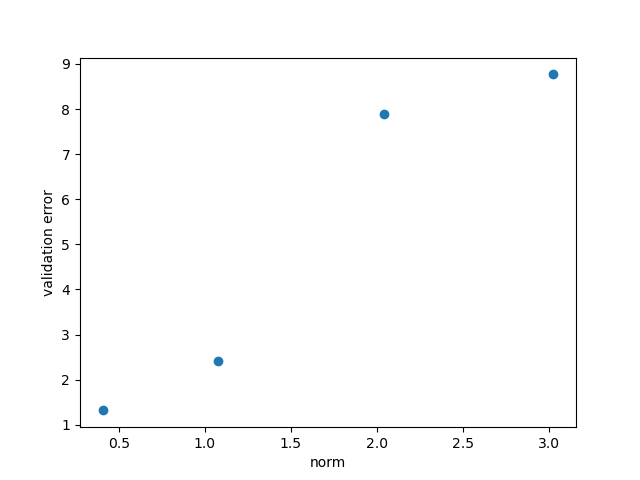
\includegraphics[width=.5\linewidth]{04-implicitreg/implicitreg_linear.png}
	\caption{Visual impaired students can access the corresponding desmos plot \href{https://www.desmos.com/calculator/b5ef1cvybm}{here}}
\end{figure}